\documentclass[conference]{IEEEtran}
\IEEEoverridecommandlockouts
% The preceding line is only needed to identify funding in the first footnote. If that is unneeded, please comment it out.
\usepackage{cite}
\usepackage{amsmath,amssymb,amsfonts}
\usepackage{algorithmic}
\usepackage{graphicx}
\usepackage{textcomp}
\usepackage{xcolor}
\usepackage{hyperref}
\usepackage{multirow}
\usepackage{colortbl}
\usepackage{caption}
\usepackage{subcaption}
\def\BibTeX{{\rm B\kern-.05em{\sc i\kern-.025em b}\kern-.08em
    T\kern-.1667em\lower.7ex\hbox{E}\kern-.125emX}}

    
\begin{document}

\title{Spla: Generalized Sparse Linear Algebra Library with Vendor-Agnostic GPUs Acceleration\\
\thanks{We would like to thank Huawei Technologies Co., Ltd for supporting this research. We are also grateful to our team and reviewers.\\}}

\author{\IEEEauthorblockN{1\textsuperscript{st} Egor Orachev}
\IEEEauthorblockA{\textit{St. Petersburg State University} \\
St. Petersburg, Russia \\
egor.orachev@gmail.com \\
0000-0002-0424-4059}
\and
\IEEEauthorblockN{2\textsuperscript{nd} Semyon Grigorev}
\IEEEauthorblockA{\textit{St. Petersburg State University} \\
St. Petersburg, Russia \\
s.v.grigoriev@spbu.ru \\
0000-0002-7966-0698}
}

\maketitle

\begin{abstract}
    Scalable high-performance graph analysis is a nontrivial challenge. 
    Usage of sparse linear algebra operations as building blocks for graph analysis algorithms, which is a core idea of GraphBLAS standard, is a promising way to attack it.
    While it is known that sparse linear algebra operations can be efficiently implemented on GPU, full GraphBLAS implementation on GPU is a nontrivial task that is almost solved by GraphBLAST project. 
    It is shown that utilization of GPUs for GraphBLAS implementation significantly improves performance. But GraphBLAST is not portable because it is based on Nvidia Cuda.
    In this work we propose Spla library which aims to solve this problem using OpenCL API for vendor-agnostic GPUs accelerated computations.
    Evaluation shows that the proposed solution demonstrates performance comparable with GraphBLAST, outperforming it up to 36 times in some cases, and remains portable across different GPUs vendors.
\end{abstract}

\begin{IEEEkeywords}
graphs, algorithms, graph analysis, sparse linear algebra, GraphBLAS, GPGPU, OpenCL
\end{IEEEkeywords}

\section*{Введение}

Все чаще современные системы аналитики и рекомендаций строятся на основе анализа данных, структурированных с использованием \textit{графовой модели}. В данной модели основные сущности представляются вершинами графа, а отношения между сущностями --- ориентированными ребрами с различными метками. Подобная модель позволяет относительно легко и практически в явном виде моделировать сложные иерархические структуры, которые не так просто представить, например, в классической \textit{реляционной модели}. В качестве основных областей применения графовой модели можно выделить следующие: графовые базы данных~\cite{article:querying_graph_databases}, анализ RDF данных~\cite{article:cfpq_and_rdf_analysis}, биоинформатика~\cite{article:rna_prediction} и статический анализ кода~\cite{article:dyck_cfl_code_analysis}.

Поскольку графовая модель используется для моделирования отношений между объектами, при решении прикладных задач возникает необходимость в выявлении более сложных взаимоотношений между объектами. Для этого чаще всего формируются запросы в специализированных программных средствах для управления графовыми базами данных. В качестве запроса можно использовать некоторый \textit{шаблон} на путь в графе, который будет связывать объекты, т.е. выражать взаимосвязь между ними. В качестве такого шаблона можно использовать формальные грамматики, например, регулярные или контекстно-свободные (КС). Используя вычислительно более выразительные грамматики, можно формировать более сложные запросы и выявлять нестандартные и скрытые ранее взаимоотношения между объектами. Например, \textit{same-generation queries}~\cite{inbook:databases_intro}, сходные с сбалансированными скобочными последовательностями Дика, могут быть выражены КС грамматиками, в отличие от регулярных.

Результатом запроса может быть множество пар объектов, между которыми существует путь в графе, удовлетворяющий заданным ограничениям. Также может возвращаться один экземпляр такого пути для каждой пары объектов или итератор всех путей, что зависит от семантики запроса. Поскольку один и тот же запрос может иметь разную семантику, требуются различные программные и алгоритмические средства для его выполнения.  

Запросы с регулярными ограничениями изучены достаточно хорошо, языковая и программная поддержка выполнения подобных запросов присутствует в некоторых в современных графовых базах данных. Однако, полноценная поддержка запросов с КС ограничениями до сих пор не представлена. Существуют алгоритмы~\cite{article:cfpq_and_rdf_analysis, article:hellings_cfpq, inproceedings:matrix_cfpq, inbook:kronecker_cfpq_adbis, article:cfpq_go_for_rdf} для вычисления запросов с КС ограничениями, но потребуется еще время, прежде чем появиться полноценная высокпроизводительная реализация одного из алгоритмов, способная обрабатывать реальные графовые данные.

Работы~\cite{inproceedings:cfpq_matrix_evaluation, inproceedings:cfqp_matrix_with_single_source} в качестве реализации алгоритма~\cite{inproceedings:matrix_cfpq} для выполнения запросов с КС ограничениями с семантикой достижимости и семантикой одного пути показывают, что возможно использовать GPGPU для выполнения наиболее вычислительно сложных частей алгоритма, что дает \textit{существенный} прирост в производительности. 

Недавно представленный алгоритм~\cite{inbook:kronecker_cfpq_adbis} для вычисления запросов с КС ограничениями полагается на операции линейной алгебры: произведение Кронекера (частный случай тензорного произведения), умножение и сложение матриц в полукольце булевой алгебры. Важной задачей является реализация данного алгоритма, так как он в сравнении с~\cite{inproceedings:cfqp_matrix_with_single_source} позволяет выполнять запросы для всех ранее упомянутых семантик, потенциально поддерживает б\'ольшие по размеру КС запросы, с незначительными накладными расходами позволяет выполнять запросы с регулярными ограничениями, а с реализацией на GPGPU позволит получить потенциально приемлемое время выполнения запрсов.
\section{Proposed Solution Description}

This section describes the high-level details of the proposed solution. 
It highlights the design principles, high-level architecture of the solution, data storage representation, operations, and also shows differences from the GraphBLAS API.

\subsection{Design Principles}

Spla library aims to address some of GraphBLAS standard limitations.
It is designed the way to maximize potential library performance, to simplify its implementation and extension, and to provide the end-user verbose, but expressive interface allowing customization and precise control over operations execution. 
These ideas are captured in the following principles.

\begin{itemize}
    \item \textit{Optional acceleration}. Library is designed in a way, that GPU acceleration is fully plugable and optional part. Library can perform computations using standard CPU pipeline. If GPU acceleration is presented, library can offload a part of a work for it. It allows both non-trivial processing of the data on the CPU only, as well as possibility to integrate different backends in the future.  
    \item \textit{User-defined functions}. The user can create custom element-wise functions to parameterize operations. Custom functions can be used for both CPU and GPU execution.
    \item \textit{Predefined scalar data types}. The library provides a set of built-in scalar data types that have a natural one-to-one relationship with native GPU built-in types. Data storage is transparent. The library interprets the data as POD-structures. The user can interpret individual elements as a sequence of bytes of a fixed size.
    \item \textit{Hybrid-storage format}. The library automates the process of data storage and preprocessing. It supports several data formats, chooses the best one depending on the situation.
    \item \textit{Exportable interface}. The library has a C++ interface with an automated reference-counting and with no-templates usage. It is compiled into a shared library. The interface is wrapped by C99 compatible API and exported to other languages, for example, in a form of a Python package.
    \item \textit{Introspection}. Each library class instantiates into a first-class object. Such objects can be captured, manipulated, passed as arguments and returned as function results. Parameterization types of containers can be inspected, as well as declared user functions.
\end{itemize}

\subsection{Architecture Overview}

The general idea of the proposed solution is depicted in Fig.~\ref{fig:design}. 
The core of the library and its main part is the CPU, which is the master node which controls all computations. 
It is responsible for storing data, maintaining a registry with algorithms, and scheduling operations to perform. 
In this paradigm, the GPU is an optional backend for acceleration, implemented through a special interface. 
It can optionally store data in a specific format. 
The CPU can offload the calculation of a part of the operations to the GPU, if the corresponding operation is supported by the given accelerator.

The reason for this is that the CPU and GPU are inherently asymmetric in nature. 
The end-user uses CPU side API. Thus, some preprocessing on the CPU side must be always done in the majority of cases. In addition, access to data on the GPU and their storage is carried out differently due to the peculiarities of the execution of kernels. 
Also, VRAM is more expensive and has less capacity than RAM.
Therefore, RAM is a cache for VRAM, and data duplication can be neglected. 
In the end, the explicit separation of the CPU side from the GPU backend gives the modularity. 
This can be used not only to support different GPU technologies, but also to integrate multiple GPUs or distributed processing in the future.

\begin{figure}[t]
\centering
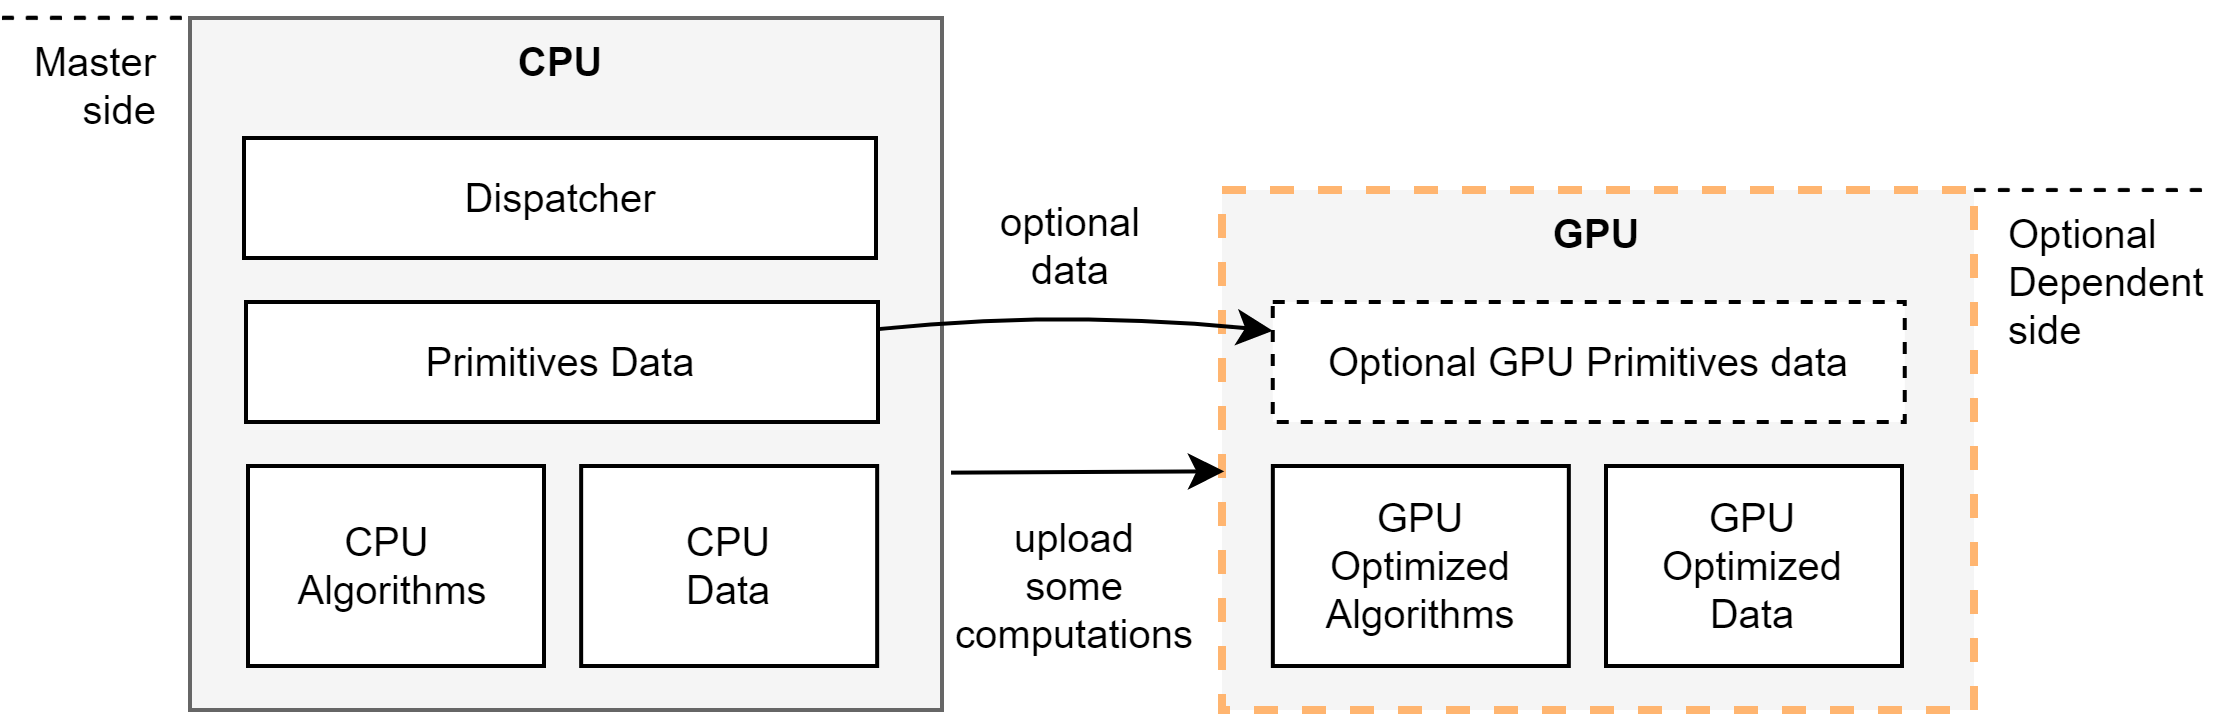
\includegraphics[width=0.95\linewidth]{figures/design_idea.png}
\caption{Proposed solution general design.}
\label{fig:design}
\end{figure}
    
\subsection{Data Containers}

Library provides general \textit{M-by-N Matrix}, \textit{N Vector}, \textit{Scalar} and \textit{N Array} data containers.
Underlying primitive value types are specified by \textit{Type} object. 
Single vector or matrix data is stored in specialized multi-format storage container. An example of the single vector storage is depicted in Fig.~\ref{fig:vec_storage}. 

The storage is responsible for keeping data in multiple different formats at the same time. 
Each format is best suited for a specific type of task and requested on demand. 
Key-value dictionary suites well frequent insertion, query or deletion operations, when memory usage and response time are critical. 
Mathematical operations perform better with compacted sequential lists of values since they have more friendly cache behaviour. 
GPU operations require separate format with a copy of the data resident in VRAM.

The storage and particular format can be inspected using array primitive. It allows one to get the view of an existing CPU or GPU buffer without actual copy, or initialize matrix or vector in particular format from existing arrays, which may be created and filled by user code. Also array gives an ability to acquire raw pointer to memory or GPU buffer handler, what can be used for interoperability and seamless integration into user data pipeline.

Data transformation from one format to another is carried out using a special rules graph. Example graph for a vector storage is shown in Fig.~\ref{fig:vec_tsf}. 
The directed edges in this graph indicate conversion rules. 
The graph must be the single strongly connected component. 
An example of the data transformation process is depicted in Fig.~\ref{fig:vec_exmp}. 
For a requested format the best path of convertation is obtained. Currently, the shortest one is used. 
Weight assignment to rules can potentially be used to prioritize convertations for some formats. 

Currently, several storage formats are supported. 
There is dictionary of keys for vector and matrix (DoK), list of coordinates (COO), dense vector, list of lists (LIL) and compressed sparse rows (CSR) matrix formats.  
Other formats, such as CSC, DCSR, ELL, etc., can be added to the library by the implementation of formats conversion and by the specialization of operations for a specific format. 

\begin{figure}[b]
\centering
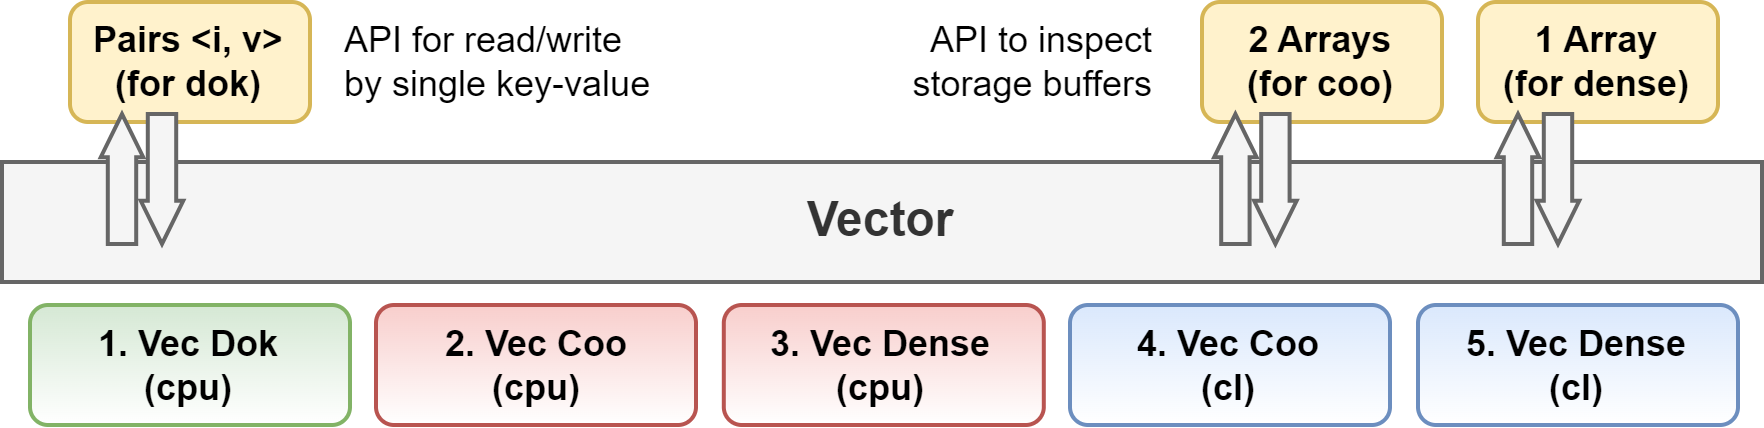
\includegraphics[width=0.8\linewidth]{figures/vector_storage.png}
\caption{Vector primitive storage holds the same data potentially in multiple different formats at the same time. Some slots can be empty.}
\label{fig:vec_storage}
\end{figure}

\begin{figure}[]
\centering
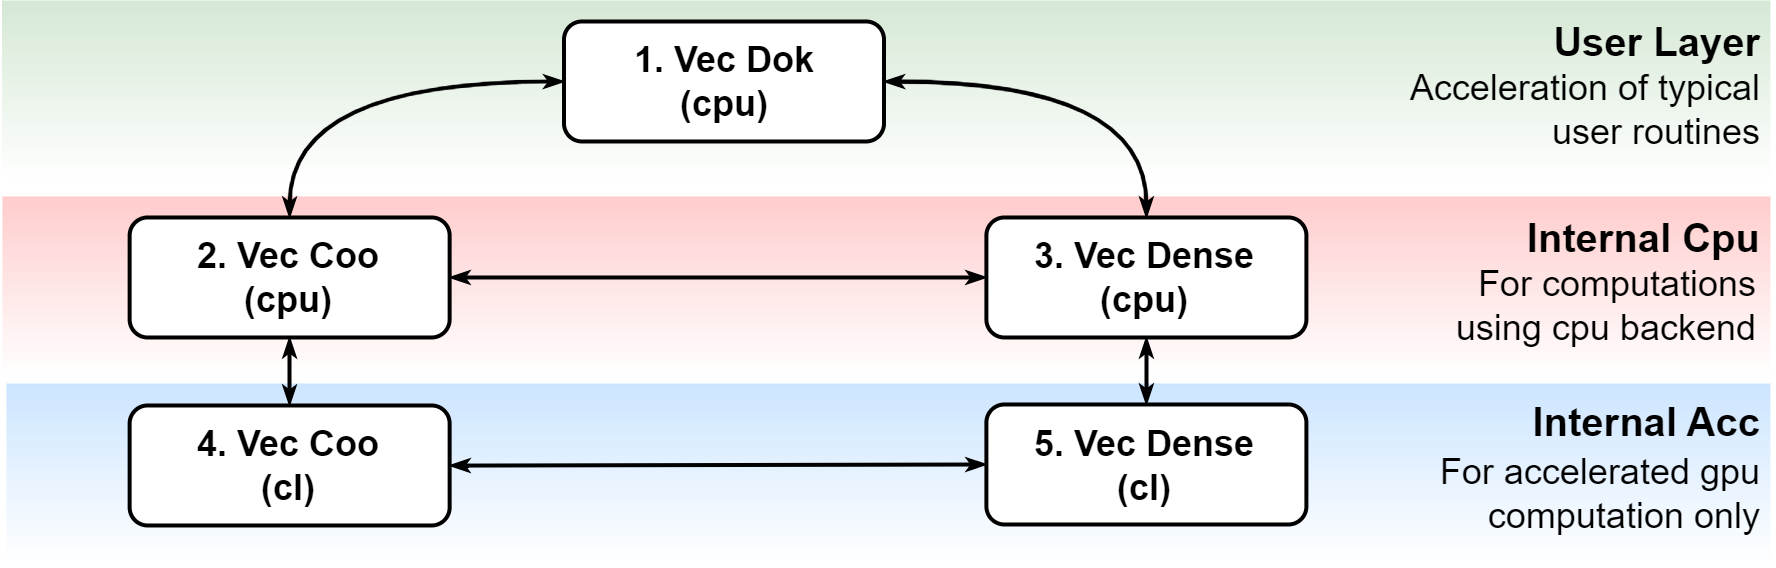
\includegraphics[width=0.8\linewidth]{figures/storage_transformation_graph.png}
\caption{Vector storage transformation graph. The graph defines how data can be obtained from one format in another.}
\label{fig:vec_tsf}
\end{figure}

\begin{figure}[]
\centering
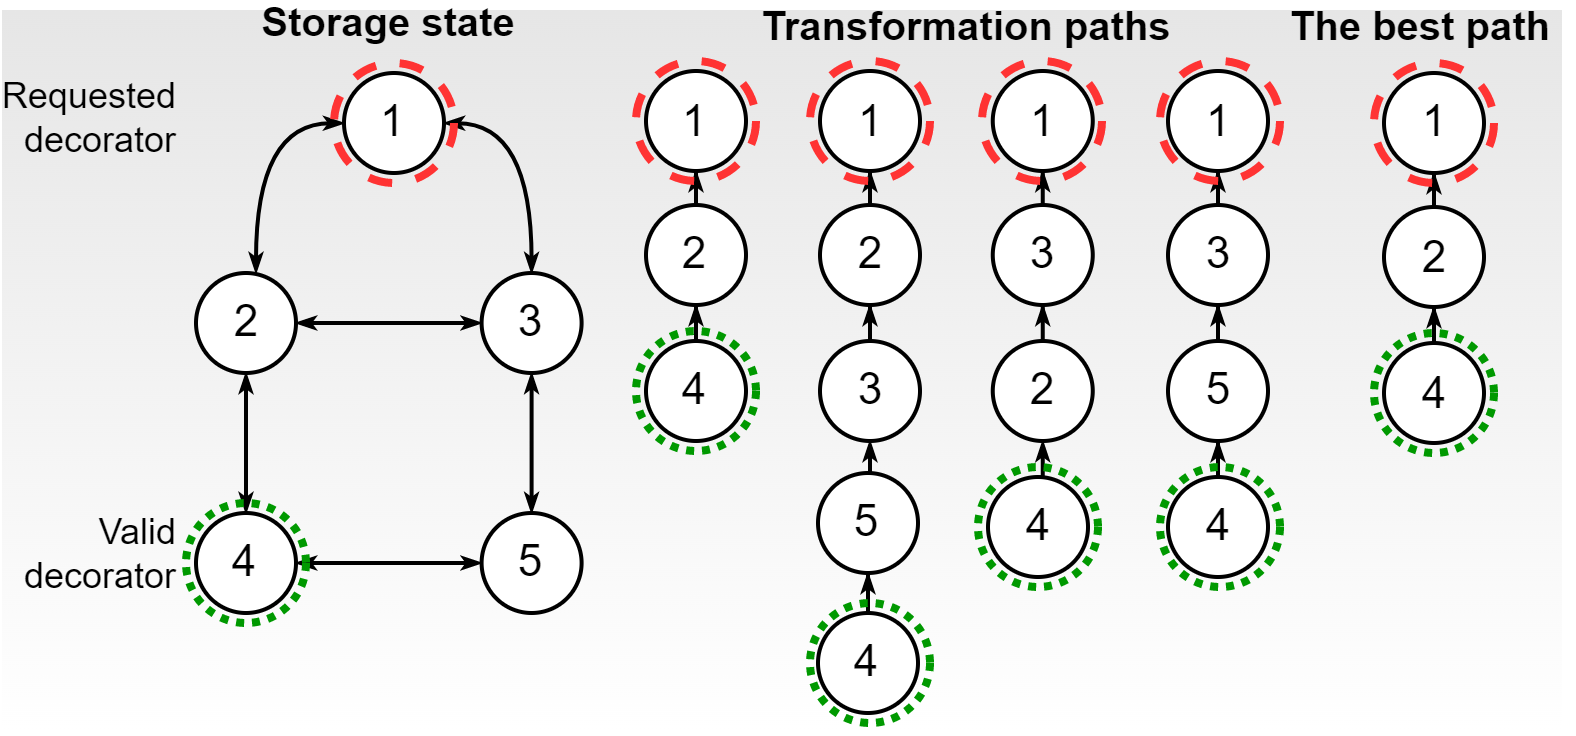
\includegraphics[width=0.8\linewidth]{figures/storage_transformation.png}
\caption{Vector storage transformation process. Green is valid format. Red is requested format. No highlight is currently invalid format.}
\label{fig:vec_exmp}
\end{figure}

\subsection{Algebraic Operations}

Library provides a number of commonly used operations, such as \textit{vxm}, \textit{mxv}, \textit{mxmT}, \textit{element-wise add}, \textit{assign}, \textit{map}, \textit{reduce}, etc.
Other operations can be added on demand.
Interface of operations is inspired by GraphBLAS standard. 
It supports \textit{masking}, parametrization by \textit{binary mult} and \textit{binary add} functions, \textit{select} for filtering and mask application, \textit{unary op} for values transformation, and \textit{descriptor} object for additional operation tweaking.

\subsection{Differences with GraphBLAS standard}

To be clear, the proposed solution is not an implementation of GraphBLAS C or C++ API. 
The design of the library uses only the concepts described by the standard. 
Thus, the signatures and semantics of some of the operations have been changed in the proposed solution. 
The API has been made more verbose and explicit. 
In particular, the handling of \textit{zero} elements and \textit{masking} are made cleaner for the end user. The library interprets data simply as collections of bytes, without mathematical semantics.
Identity element must be explicitly passed by the user where required. Mask applied using separate user-defined predicate for selection. Special fill value used for sparse-dense convertations. It allows to make the memory usage predictable and the result of each operation clear to the end user without internal implicit storage manipulations.
\section{Evaluation}

For performance analysis of the proposed solution, a few most common graph algorithms were evaluated using real-world sparse matrix data. 
The following tools for comparison were chosen: LaGraph~\cite{misc:la_graph}~(ver. Feb 13, 2022) in connection with SuiteSparse~\cite{article:suite_sparse_for_graph_problems}~(ver. Jan 14, 2022) as a baseline CPU tool, Gunrock~\cite{article:gunrock}~(ver. Nov 7, 2021) and GraphBLAST~\cite{yang2019graphblast}~(ver. Jun 18, 2021) as a Nvidia GPU tools. 
Also, algorithms were tested on several devices with distinct OpenCL vendors in order to validate the portability of the proposed solution. 

\subsection{Research questions}

In general, these evaluation intentions are summarized in the following research questions. 

\vspace{0.2cm}
\begin{itemize}
    \item[\textbf{RQ1}] What is the performance of the proposed solution relative to existing tools for GPU analysis?

    \item[\textbf{RQ2}] What is the performance of the proposed solution on various devices vendors and OpenCL runtimes?

    \item[\textbf{RQ3}] What is the performance of the proposed solution on integrated GPU compared to existing CPU tool for analysis?
\end{itemize}

\subsection{Evaluation setup}

\textbf{For evaluation of RQ1}, a PC with Ubuntu 20.04 installed used, which has 3.40Hz Intel Core i7-6700 4-core CPU, DDR4 64Gb RAM, Intel HD Graphics 530 integrated GPU, and Nvidia GeForce GTX 1070 dedicated GPU with 8Gb on-board VRAM. 

\textbf{For evaluation of RQ2}, a PC with Ubuntu 22.04 installed used, which has 4.70Hz AMD Ryzen 9 7900x 12-core CPU, DDR4 128 GB RAM, AMD GFX1036 integrated GPU, and either Intel Arc A770 flux dedicated GPU with 8GB on-board VRAM or AMD Radeon Vega Frontier Edition dedicated GPU with 16GB on-board VRAM.

\textbf{For evaluation of RQ3}, the first PC with Intel CPU and integrated GPU and the second PC with AMD CPU and integrated GPU are used.

Spla and LaGraph were compiled with GCC v9.4. Gunrock and GraphBLAST were compiled with GCC v8.4 and Nvidia NVCC v10.1.
Release mode and maximum optimizations level were enabled for all tested programs. 

\subsection{Methodology}

All tests are averaged across 10 runs. The deviation of measurements does not exceed the threshold of 10 percent. Additional warm-up run for each test execution is excluded from measurements. 

Only actual execution time of algorithms is measured. Data loading time, preparation, format transformations, and host-device initial communications are excluded from time measurements. 

The graph vertex with index 1 is set as the initial traversal vertex in the algorithms BFS and SSSP for all tested instruments and all tested devices.

For measurements standard official benchmarks are used, which provided by compared tools developers. These benchmarks are intended for performance comparison. Thus, all tools agree on measurements, what is clearly seen from the source code of those benchmarks.

\subsection{Graph algorithms}

For preliminary study \textit{breadth-first search} (BFS), \textit{single-source shortest paths} (SSSP), \textit{page rank} (PR) and \textit{triangles counting} (TC) algorithms were chosen.
Implementation of those algorithms for competitors is used from official source code repositories with default parameters. Compared tools are allowed to make any optimizations as long as the result remains correct.

\subsection{Dataset}

\begin{table}[tbp]
\caption{Dataset description.} 
\begin{center}
    \begin{tabular}{|l|r|r|r|r|r|}
    \hline
    \multirow{2}{*}{Graph} & \multirow{2}{*}{Vertices} & \multirow{2}{*}{Edges} & \multicolumn{3}{c|}{Out Degree} \\ 
    \cline{4-6} & & & \multicolumn{1}{r|}{Avg} & \multicolumn{1}{r|}{Sd} & \multicolumn{1}{r|}{Max} \\
    \hline
    \hline
    \rowcolor{black!10} coAuthorsCit&227.3K&1.6M&7.2&10.6&1.4K\\
    \rowcolor{black!2 } coPapersDBLP&540.5K&30.5M&56.4&66.2&3.3K\\
    \rowcolor{black!10} amazon2008&735.3K&7.0M&9.6&7.6&1.1K\\
    \rowcolor{black!2 } hollywood2009&1.1M&112.8M&98.9&271.9&11.5K\\
    \rowcolor{black!10} comOrkut&3.1M&234.4M&76.3&154.8&33.3K\\
    \rowcolor{black!2 } citPatents&3.8M&33.0M&8.8&10.5&793.0\\
    \rowcolor{black!10} socLiveJournal&4.8M&85.7M&17.7&52.0&20.3K\\
    \rowcolor{black!2 } indochina2004&7.4M&302.0M&40.7&329.6&256.4K\\
    \hline
    \rowcolor{black!10} belgiumosm&1.4M&3.1M&2.2&0.5&10.0\\
    \rowcolor{black!2 } roadNetCA&2.0M&5.5M&2.8&1.0&12.0\\
    \rowcolor{black!10} rggn222s0&4.2M&60.7M&14.5&3.8&36.0\\
    \rowcolor{black!2 } rggn223s0&8.4M&127.0M&15.1&3.9&40.0\\
    \rowcolor{black!10} roadcentral&14.1M&33.9M&2.4&0.9&8.0\\
    \hline
    \end{tabular}
    \label{dataset:info}
\end{center}
\end{table}

Thirteen matrices with graph data were selected from the Sparse Matrix Collection at University of Florida~\cite{dataset:sparse_matrix_collection}. Information about graphs is summarized in Table~\ref{dataset:info}. This is a common graphs collection used for sparse linear algebra and graph algorithms benchmarks in other works in the domain. These graphs represents typical analysed data structure, sparsity, distribution, and allows one to study common behaviour and performance characteristics of developed libraries.

The dataset is converted to undirected graphs. Self-loops and duplicated edges are removed. Average, sd and max metrics relate to out degree property of the vertices. For SSSP weights are initialized using pseudo-random generator with uniform $[0, 1]$ distribution of floating-point values.

Graphs are roughly divided into two groups. The first group represents relatively dense graphs, where the number of edges per node is sufficient on average to effectively load the GPU with useful work. The second group represents relatively sparse graphs, where the average vertex degree is below the typical GPU vector register size, and the search depth reaches hundreds of hoops. Graphs are sorted in ascending order by the number of vertices within each group.

\subsection{Results Summary}

\begin{figure*}[tbp]
\centering
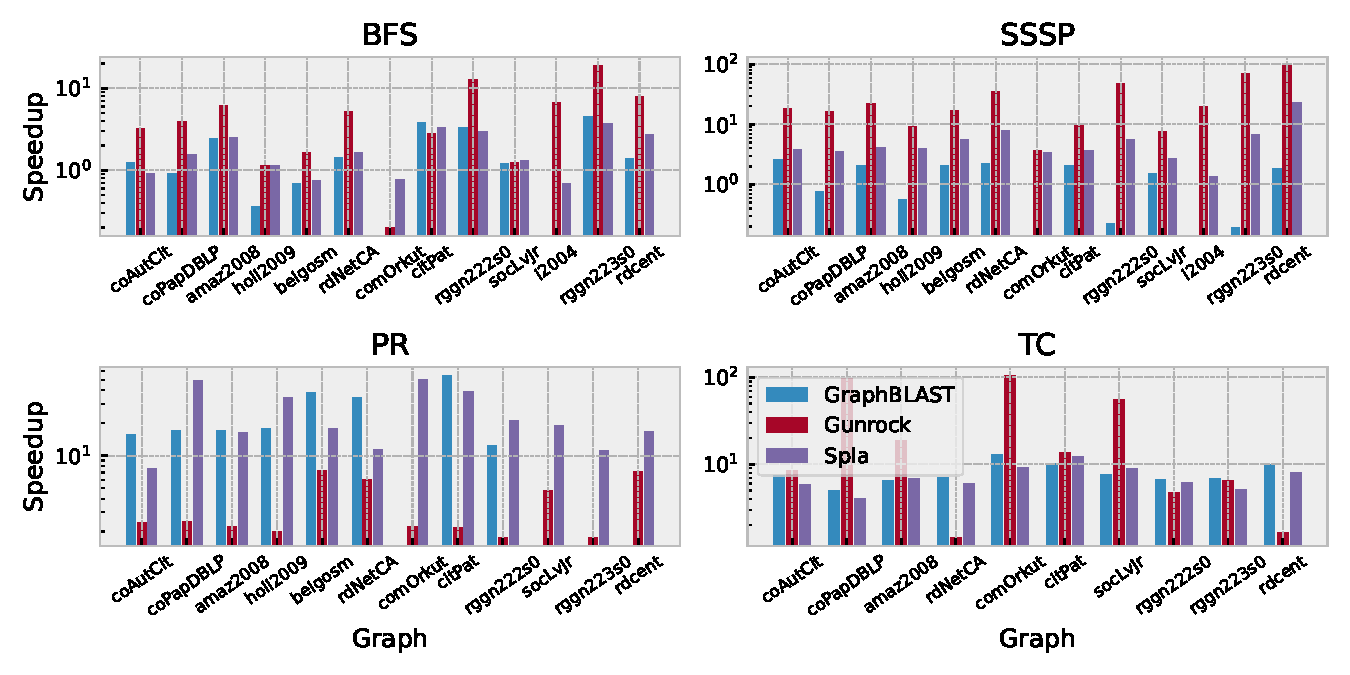
\includegraphics[width=1.0\linewidth]{plots/rq1_rel.pdf}
\caption{Performance of Spla library and GPU tools on the same device compared to LaGraph. Logarithmic scale is used.}
\label{fig:rq1_chart}
\end{figure*}

\begin{figure*}[tbp]
\centering
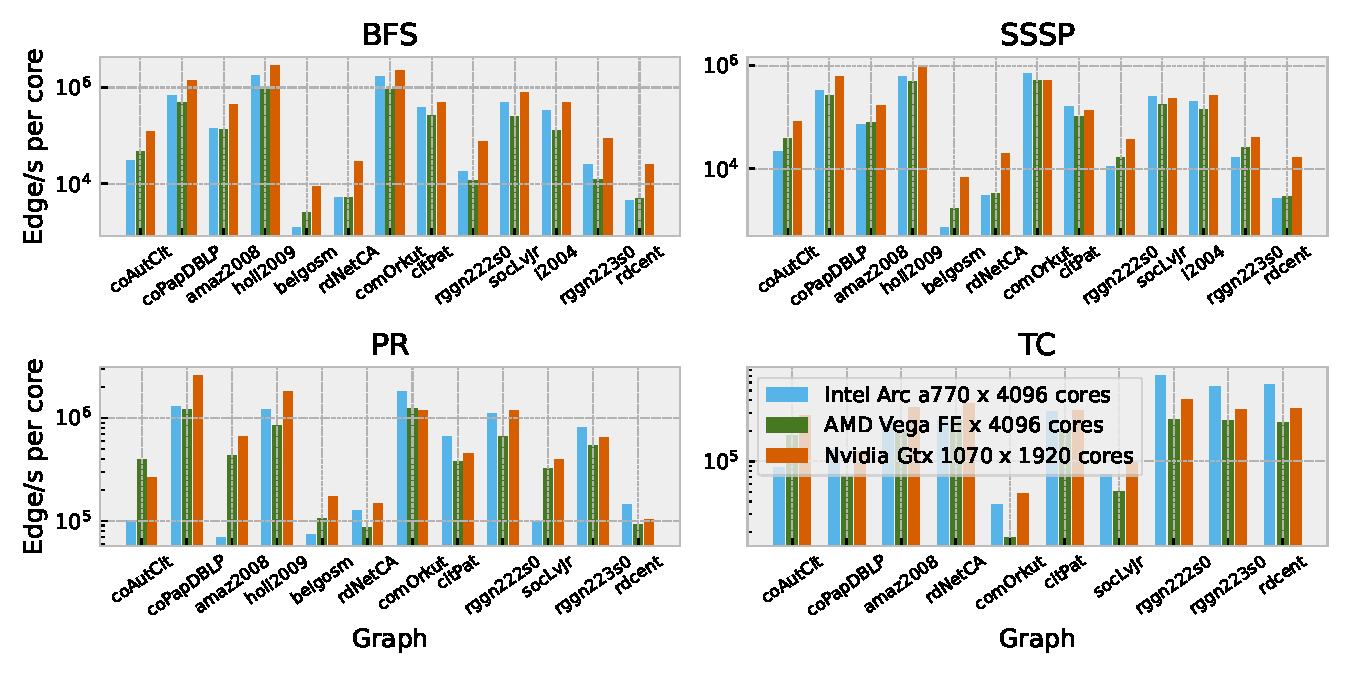
\includegraphics[width=1.0\linewidth]{plots/rq2_cores.pdf}
\caption{Performance of Spla library on different devices relative to the number of compute cores. Logarithmic scale is used.}
\label{fig:rq2_chart}
\end{figure*}

\begin{figure*}[tbp]
\centering
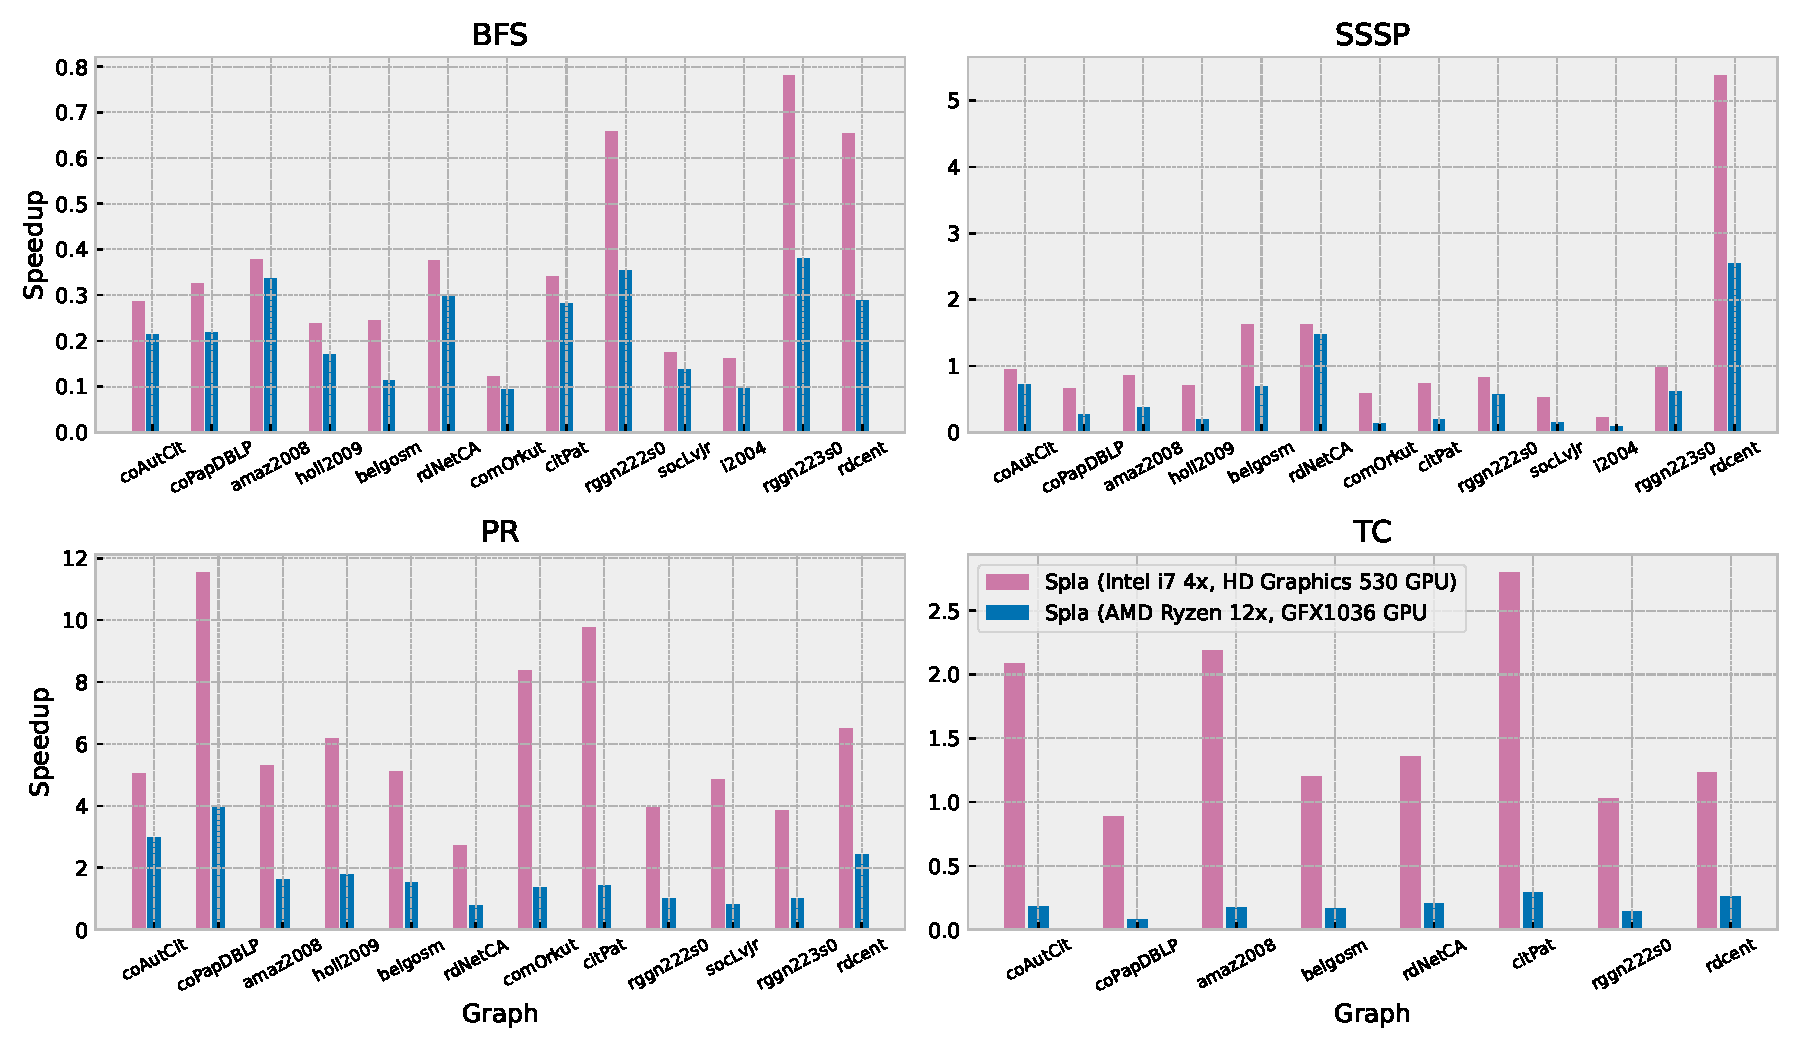
\includegraphics[width=1.0\linewidth]{plots/rq3_int.pdf}
\caption{Performance of Spla library on integrated GPU compared to LaGraph on the same chip.}
\label{fig:rq3_chart}
\end{figure*}

Fig.~\ref{fig:rq1_chart} presents results of the evaluation and compares the performance of Spla against other Nvidia GPU tools and uses as a baseline LaGraph CPU tool. 
Fig.~\ref{fig:rq2_chart} presents result of the portability analysis of the proposed solution. It shows performance of the proposed solution on discrete GPUs of distinct vendors.
Fig.~\ref{fig:rq3_chart} present result of per-device comparison of Spla library running on integrated GPU and CPU LaGraph running on the same chip. 

The absolute results of the performance study are available in the Table~\ref{rq1_table}, Table~\ref{rq2_table} and Table~\ref{rq3_table} for each stated research question. Cells left with \textit{none} if tool failed to analyze graph due to \textit{out of memory} exception.\\

\textit{RQ1. What is the performance of the proposed solution relative to existing tools for GPU analysis?} In general, Spla shows very acceptable performance in all algorithms, running with comparable speed to its nearest competitor, GraphBLAST. Also proposed library does not suffer from memory issues on some large graphs such as \textit{indochina}, \textit{orkut} and \textit{rggn23}. Spla is consistently several times faster than LaGraph, overcoming it up to $25\times$ in some cases. Gunrock is the fastest GPU framework for analysis. It dominates the overall performance and only suffers in a PR algorithm.

Taking a closer look at Fig.~\ref{fig:rq1_chart}, Spla-based BFS shows comparable to GraphBLAST performance in most cases. Spla has good speed at relatively dense graphs with high vertex degree and small depth of the search, what allows to saturate GPU with a work better. However, the performance degrades in network and road graphs with small front of the search and large diameter, what cause a lot of iterations. Thus, both Spla and GraphBLAST suffer from the overhead of kernel launches and relatively small amount of the work for a GPU. SSSP shares with BFS the same picture in general. However, Spla behaves here slightly better than GraphBLAST, running up to $36\times$ faster at some extreme cases.

For PR, Spla and GraphBLAST show the best performance, except cases with GraphBLAST memory issues. Both tools are faster than Gunrock in average reaching up to $20\times$ and more relative speedup. This performance can be motivated by the usage of \textit{mxv} operation as a core primitive for pull-updates, which is computationally intensive and has good work load balance compared to Gunrock push-updates. However, Spla suffers a bit in case of lower-degree graphs due to lack of more precise balance for small matrix rows.

Finally, Gunrock dominates performance in TC as well, except two sparse road graphs where it has significant performance drop down. Spla and GraphBLAST have comparable results. However, GraphBLAST slightly faster nearly in all runs. Both tools use the same approach for \textit{mxm} implementation. However, Spla may encounter some OpenCL overhead or lack of precise performance tuning.\\

\textit{RQ2. What is the performance of the proposed solution on various devices vendors and OpenCL runtimes?} Spla successfully launches and workes on the GPU of distinct vendors, including Intel, AMD and Nvidia. It shows promising performance and demonstrated scalability in relation to the number of computing cores. Fig.~\ref{fig:rq2_chart} depicts the edge/s throughput per a GPU core for all devices. This metric is quite predictable for the same graphs. This can be seen if one takes into account the overall shape of the figures for BFS, SSSP and PR as a whole.

In general, Spla on Nvidia shows better average performance, especially for sparser graphs with relatively small degree per row. Nvidia OpenCL driver features faster memory allocations and has less overhead on a frequent kernel launches. Spla on Intel runtime lags a bit behind Nvidia, but performs better in some PR and TC cases. Spla performance on AMD is acceptable. However, better tuning and further polishing are required.\\

\textit{RQ3. What is the performance of the proposed solution on integrated GPU compared to existing CPU tool for analysis?} Result of detailed comparison are shown in Fig.~\ref{fig:rq3_chart}. This figure depict Spla relative to LaGraph speedup on the same chip, where Spla is running on integrated GPU part and LaGraph is running on multi-core CPU part. 

In general, LaGraph shows better performance for both CPUs, especially on a new powerful AMD Ryzen with 12 cores. The difference in a speed is extremely dramatic in BFS and SSSP algorithms. For a PR algorithm the picture is slightly better. Spla shows up to $10\times$ speedup. PR algorithm tends to be more computationally intensive, so difference to BFS and SSSP is reasonable. For TC Spla performs better only for Intel device, having in some cases conservative $2\times$ speedup.\\

Summarizing, the evaluation of the proposed solution for some real-world graph data in four different algorithms shows, that OpenCL-based solution has a promising performance, comparable to analogs, has acceptable scalability on devices of different GPU vendors, and, surprisingly, has a speedup in some cases when compared with highly-optimized CPU library on some integrated GPUs. However, there are still a plenty of research questions and directions for improvement.

\begin{table}[tbp]
    \caption{RQ1. Performance comparison of the proposed solution. Time in milliseconds (lower is better).} 
    \begin{center}
        \scalebox{0.7}{
        \begin{tabular}{|l|r|r|r|r|}
        \hline
        Dataset & GraphBLAST & Gunrock & LaGraph & Spla (proposed) \\
        \hline
        \hline
        \multicolumn{5}{|c|}{BFS} \\
        \hline
        \rowcolor{black!10} coAuthorsCit&5.0&1.9&6.3&6.9\\
        \rowcolor{black!2 } coPapersDBLP&19.9&4.5&18.0&11.5\\
        \rowcolor{black!10} amazon2008&8.3&3.3&20.4&8.1\\
        \rowcolor{black!2 } hollywood2009&64.3&20.3&23.4&20.3\\
        \rowcolor{black!10} belgiumosm&200.6&84.4&138.0&181.2\\
        \rowcolor{black!2 } roadNetCA&116.3&32.4&168.2&101.7\\
        \rowcolor{black!10} comOrkut& none&205.0&40.6&53.2\\
        \rowcolor{black!2 } citPatents&30.6&41.3&115.9&35.1\\
        \rowcolor{black!10} rggn222s0&367.3&95.9&1228.1&415.3\\
        \rowcolor{black!2 } socLiveJournal&63.1&61.0&75.5&57.1\\
        \rowcolor{black!10} indochina2004& none&33.3&224.6&328.7\\
        \rowcolor{black!2 } rggn223s0&615.3&146.2&2790.0&754.9\\
        \rowcolor{black!10} roadcentral&1383.4&243.8&1951.0&710.2\\
        \hline
        \hline
        \multicolumn{5}{|c|}{SSSP} \\
        \hline
        \rowcolor{black!10} coAuthorsCit&14.7&2.1&38.9&10.3\\
        \rowcolor{black!2 } coPapersDBLP&118.6&5.6&92.2&25.7\\
        \rowcolor{black!10} amazon2008&43.4&4.0&90.0&21.7\\
        \rowcolor{black!2 } hollywood2009&404.3&24.6&227.7&57.5\\
        \rowcolor{black!10} belgiumosm&650.2&81.1&1359.8&240.9\\
        \rowcolor{black!2 } roadNetCA&509.7&32.4&1149.3&147.9\\
        \rowcolor{black!10} comOrkut& none&219.0&806.5&241.0\\
        \rowcolor{black!2 } citPatents&226.9&49.8&468.5&129.3\\
        \rowcolor{black!10} rggn222s0&21737.8&101.9&4808.8&865.4\\
        \rowcolor{black!2 } socLiveJournal&346.4&69.2&518.0&189.5\\
        \rowcolor{black!10} indochina2004& none&40.8&821.9&596.6\\
        \rowcolor{black!2 } rggn223s0&59015.7&161.1&11149.9&1654.8\\
        \rowcolor{black!10} roadcentral&13724.8&267.0&25703.4&1094.3\\
        \hline
        \hline
        \multicolumn{5}{|c|}{PR} \\
        \hline
        \rowcolor{black!10} coAuthorsCit&1.6&10.0&24.3&3.2\\
        \rowcolor{black!2 } coPapersDBLP&17.6&120.2&297.6&6.1\\
        \rowcolor{black!10} amazon2008&5.2&40.6&89.8&5.5\\
        \rowcolor{black!2 } hollywood2009&62.9&559.5&1111.2&32.4\\
        \rowcolor{black!10} belgiumosm&4.4&22.9&167.6&9.4\\
        \rowcolor{black!2 } roadNetCA&6.6&37.7&225.8&19.6\\
        \rowcolor{black!10} comOrkut& none&2333.6&5239.0&103.3\\
        \rowcolor{black!2 } citPatents&27.0&686.1&1487.0&38.3\\
        \rowcolor{black!10} rggn222s0&45.2&320.0&563.5&26.6\\
        \rowcolor{black!2 } socLiveJournal& none&445.9&2122.5&112.0\\
        \rowcolor{black!10} rggn223s0& none&662.7&1155.6&103.4\\
        \rowcolor{black!2 } roadcentral& none&408.8&2899.9&172.0\\
        \hline
        \hline
        \multicolumn{5}{|c|}{TC} \\
        \hline
        \rowcolor{black!10} coAuthorsCit&2.3&2.0&17.3&3.0\\
        \rowcolor{black!2 } coPapersDBLP&105.2&5.3&520.8&128.4\\
        \rowcolor{black!10} amazon2008&11.2&3.9&73.9&10.8\\
        \rowcolor{black!2 } roadNetCA&6.5&32.4&46.0&7.7\\
        \rowcolor{black!10} comOrkut&1776.9&218.0&23103.8&2522.0\\
        \rowcolor{black!2 } citPatents&65.5&49.7&675.0&54.5\\
        \rowcolor{black!10} socLiveJournal&504.3&69.2&3886.7&437.8\\
        \rowcolor{black!2 } rggn222s0&73.2&101.3&484.5&77.7\\
        \rowcolor{black!10} rggn223s0&151.4&158.9&1040.1&204.2\\
        \rowcolor{black!2 } roadcentral&42.6&259.3&425.3&52.7\\
        \hline
        \end{tabular}
        }
        \label{rq1_table}
    \end{center}
    \end{table}
    
    \begin{table}[tbp]
    \caption{RQ2. Portability of the proposed solution. Time in milliseconds (lower is better).} 
    \begin{center}
        \scalebox{0.7}{
        \begin{tabular}{|l|r|r|r|}
        \hline
        Dataset & Intel Arc A770 & AMD Vega Frnt. Edt. & Nvidia Gtx 1070\\
        \hline
        \hline
        \multicolumn{4}{|c|}{BFS} \\
        \hline
        \rowcolor{black!10} coAuthorsCit&12.8&8.3&6.9\\
        \rowcolor{black!2 } coPapersDBLP&10.8&14.9&11.5\\
        \rowcolor{black!10} amazon2008&12.3&12.6&8.1\\
        \rowcolor{black!2 } hollywood2009&15.3&26.7&20.3\\
        \rowcolor{black!10} belgiumosm&627.5&292.4&181.2\\
        \rowcolor{black!2 } roadNetCA&265.5&259.8&101.7\\
        \rowcolor{black!10} comOrkut&33.2&63.6&53.2\\
        \rowcolor{black!2 } citPatents&21.0&30.3&35.1\\
        \rowcolor{black!10} rggn222s0&825.3&1259.7&415.3\\
        \rowcolor{black!2 } socLiveJournal&43.0&85.8&57.1\\
        \rowcolor{black!10} indochina2004&220.6&573.4&328.7\\
        \rowcolor{black!2 } rggn223s0&1245.5&2519.6&754.9\\
        \rowcolor{black!10} roadcentral&1864.9&1680.8&710.2\\
        \hline
        \hline
        \multicolumn{4}{|c|}{SSSP} \\
        \hline
        \rowcolor{black!10} coAuthorsCit&18.3&10.4&10.3\\
        \rowcolor{black!2 } coPapersDBLP&22.9&27.7&25.7\\
        \rowcolor{black!10} amazon2008&23.4&22.2&21.7\\
        \rowcolor{black!2 } hollywood2009&44.6&56.2&57.5\\
        \rowcolor{black!10} belgiumosm&1085.9&454.8&240.9\\
        \rowcolor{black!2 } roadNetCA&447.3&422.5&147.9\\
        \rowcolor{black!10} comOrkut&79.7&111.5&241.0\\
        \rowcolor{black!2 } citPatents&49.8&78.4&129.3\\
        \rowcolor{black!10} rggn222s0&1378.8&924.3&865.4\\
        \rowcolor{black!2 } socLiveJournal&82.7&120.7&189.5\\
        \rowcolor{black!10} indochina2004&366.2&519.0&596.6\\
        \rowcolor{black!2 } rggn223s0&1880.2&1201.4&1654.8\\
        \rowcolor{black!10} roadcentral&3176.3&2848.8&1094.3\\
        \hline
        \hline
        \multicolumn{4}{|c|}{PR} \\
        \hline
        \rowcolor{black!10} coAuthorsCit&3.9&1.0&3.2\\
        \rowcolor{black!2 } coPapersDBLP&5.7&6.1&6.1\\
        \rowcolor{black!10} amazon2008&25.2&4.0&5.5\\
        \rowcolor{black!2 } hollywood2009&22.6&32.4&32.4\\
        \rowcolor{black!10} belgiumosm&10.2&7.1&9.4\\
        \rowcolor{black!2 } roadNetCA&10.8&15.7&19.6\\
        \rowcolor{black!10} comOrkut&31.9&46.6&103.3\\
        \rowcolor{black!2 } citPatents&12.3&21.3&38.3\\
        \rowcolor{black!10} rggn222s0&13.4&22.4&26.6\\
        \rowcolor{black!2 } socLiveJournal&210.0&64.2&112.0\\
        \rowcolor{black!10} rggn223s0&38.6&57.2&103.4\\
        \rowcolor{black!2 } roadcentral&57.9&89.6&172.0\\
        \hline
        \hline
        \multicolumn{4}{|c|}{TC} \\
        \hline
        \rowcolor{black!10} coAuthorsCit&4.6&2.2&3.0\\
        \rowcolor{black!2 } coPapersDBLP&57.6&106.2&128.4\\
        \rowcolor{black!10} amazon2008&6.9&8.5&10.8\\
        \rowcolor{black!2 } roadNetCA&5.4&5.4&7.7\\
        \rowcolor{black!10} comOrkut&1533.5&3267.6&2522.0\\
        \rowcolor{black!2 } citPatents&25.9&39.8&54.5\\
        \rowcolor{black!10} socLiveJournal&280.6&420.3&437.8\\
        \rowcolor{black!2 } rggn222s0&21.0&57.8&77.7\\
        \rowcolor{black!10} rggn223s0&56.7&123.2&204.2\\
        \rowcolor{black!2 } roadcentral&14.5&34.6&52.7\\
        \hline
        \end{tabular}
        }
        \label{rq2_table}
    \end{center}
    \end{table}
    
    \begin{table}[tbp]
    \caption{RQ3. Integrated GPU mode performance comparison of the proposed solution. Time in milliseconds (lower is better).} 
    \begin{center}
        \scalebox{0.7}{
        \begin{tabular}{|l|r|r|r|r|}
        \hline
        \multirow{2}{*}{Dataset} & \multicolumn{2}{c|}{Intel i7, HD Graphics 530} & \multicolumn{2}{c|}{AMD Ryzen 9, GFX1036} \\
        \cline{2-5}
        & LaGraph & Spla (proposed) & LaGraph & Spla (proposed) \\
        \hline
        \hline
        \multicolumn{5}{|c|}{BFS} \\
        \hline
        \rowcolor{black!10} coAuthorsCit&7.5&26.3&3.9&18.2\\
        \rowcolor{black!2 } coPapersDBLP&18.7&57.3&12.0&54.9\\
        \rowcolor{black!10} amazon2008&24.6&65.0&13.5&40.0\\
        \rowcolor{black!2 } hollywood2009&23.8&100.1&14.8&86.6\\
        \rowcolor{black!10} belgiumosm&131.4&536.0&60.0&527.6\\
        \rowcolor{black!2 } roadNetCA&173.2&461.8&100.8&339.7\\
        \rowcolor{black!10} comOrkut&41.6&341.4&25.2&269.4\\
        \rowcolor{black!2 } citPatents&126.9&371.6&61.3&217.7\\
        \rowcolor{black!10} rggn222s0&1288.0&1959.9&644.6&1821.7\\
        \rowcolor{black!2 } socLiveJournal&75.0&429.8&41.6&301.6\\
        \rowcolor{black!10} indochina2004&228.5&1424.8&137.0&1445.1\\
        \rowcolor{black!2 } rggn223s0&2850.8&3647.2&1403.9&3701.3\\
        \rowcolor{black!10} roadcentral&2087.8&3196.3&767.2&2670.3\\
        \hline
        \hline
        \multicolumn{5}{|c|}{SSSP} \\
        \hline
        \rowcolor{black!10} coAuthorsCit&40.5&42.5&29.2&40.5\\
        \rowcolor{black!2 } coPapersDBLP&92.9&141.8&48.9&181.6\\
        \rowcolor{black!10} amazon2008&97.4&114.4&48.3&131.3\\
        \rowcolor{black!2 } hollywood2009&236.7&337.9&93.8&507.4\\
        \rowcolor{black!10} belgiumosm&1383.2&854.3&588.9&845.7\\
        \rowcolor{black!2 } roadNetCA&1174.2&721.7&712.7&482.9\\
        \rowcolor{black!10} comOrkut&822.9&1420.5&214.8&1699.5\\
        \rowcolor{black!2 } citPatents&488.3&669.4&171.4&897.3\\
        \rowcolor{black!10} rggn222s0&4919.1&5928.3&2845.6&4952.9\\
        \rowcolor{black!2 } socLiveJournal&534.7&1007.7&185.3&1205.1\\
        \rowcolor{black!10} indochina2004&837.1&3708.3&345.5&3971.8\\
        \rowcolor{black!2 } rggn223s0&11375.6&11567.8&6099.6&9899.7\\
        \rowcolor{black!10} roadcentral&26314.1&4887.0&7867.2&3102.0\\
        \hline
        \hline
        \multicolumn{5}{|c|}{PR} \\
        \hline
        \rowcolor{black!10} coAuthorsCit&25.3&5.0&17.6&5.9\\
        \rowcolor{black!2 } coPapersDBLP&302.3&26.2&154.5&39.0\\
        \rowcolor{black!10} amazon2008&93.0&17.5&36.0&22.4\\
        \rowcolor{black!2 } hollywood2009&1109.8&179.9&531.7&300.7\\
        \rowcolor{black!10} belgiumosm&178.9&35.0&45.1&29.4\\
        \rowcolor{black!2 } roadNetCA&236.9&86.9&67.6&86.2\\
        \rowcolor{black!10} comOrkut&4458.5&531.9&959.6&701.4\\
        \rowcolor{black!2 } citPatents&1559.9&159.8&277.4&195.7\\
        \rowcolor{black!10} rggn222s0&576.7&145.9&275.1&270.2\\
        \rowcolor{black!2 } socLiveJournal&2181.0&449.7&520.5&630.9\\
        \rowcolor{black!10} rggn223s0&1187.0&309.3&617.2&605.3\\
        \rowcolor{black!2 } roadcentral&2995.8&461.4&993.7&409.8\\
        \hline
        \hline
        \multicolumn{5}{|c|}{TC} \\
        \hline
        \rowcolor{black!10} coAuthorsCit&17.3&8.3&5.2&28.3\\
        \rowcolor{black!2 } coPapersDBLP&534.1&604.2&129.4&1682.3\\
        \rowcolor{black!10} amazon2008&75.4&34.5&22.2&126.6\\
        \rowcolor{black!2 } belgiumosm&28.1&23.4&11.3&67.8\\
        \rowcolor{black!10} roadNetCA&47.7&35.2&21.5&105.6\\
        \rowcolor{black!2 } citPatents&693.1&247.6&170.5&589.3\\
        \rowcolor{black!10} rggn222s0&495.2&481.3&177.7&1218.1\\
        \rowcolor{black!2 } roadcentral&438.8&355.8&176.6&679.7\\
        \hline
        \end{tabular}
        }
        \label{rq3_table}
    \end{center}
    \end{table}  
\section{Заключение}

В рамках выполнения данной работы были получены следующие результаты:

\begin{itemize}
    \item Спроектирована библиотека примитивов линейной булевой алгебры для работы с разреженными данными на GPGPU. Данная библиотека экспортирует С-совместимый интерфейс, имеет поддержку различных вычислительных модулей, а также предоставляет модуль для работы конечного пользователя с примитивами библиотеки в высокоуровневой среде вычислений с управляемыми ресурсами.

    \item Реализована библиотека cuBool в соответствии с разработанной архитектурой. Ядро библиотеки написано на языке С++, а математические операции, выполняющиеся на GPGPU, реализованы на языке CUDA C/C++. Библиотека предоставляет модуль CPU вычислений для компьютеров без Cuda девайсов. Также создан Python-пакет pycubool, который позволяет использовать функциональность библиотеки в среде Python. Данный пакет доступен для скачивания через пакетный менеджер PyPI.
    
    \item Реализован алгоритм поиска путей с КС ограничениями через тензорное произведение с использованием Python пакета разработанной библиотеки. Данный алгоритм использует операции матричного умножения, сложения и произведение Кронекера в булевом полукольце, а также различные операции для манипуляций над значениями матриц. На вход алгоритм получается представление графа и КС грамматики в виде набора матриц, а на выходе --- возвращает матрицу смежности графа достижимости, а также индекс, который позволяет восстанавливать все пути в графе, в соответствии с входной грамматикой.
    
    \item Выполнено экспериментальное исследование реализованной библиотеки с использованием синтетических и реальных данных из коллекции Разреженных Матриц Университета Флориды. Замеры производительности операции матричного умножения показывают ускорение до 5 раз в сравнении с существующими аналогами при меньшем потреблении памяти. Матричное умножение сравнимо по времени с существующими аналогами, однако потребляет меньше памяти. Также выполнено экспериментальное исследование производительности реализованного алгоритма и его сравнение с существующими алгоритмами для выполнения КС запрос. В качестве данных для замеров использовалась коллекция RDF и синтетических данных Лаборатории Языковых Инструментов JetBrains Research. Замеры показали что (этого мы пока не знаем).
\end{itemize}

На основе результатов, полученных в данном иследовании, была написана статья, принятая на конференцию GrAPL 2021\footnote{GrAPL 2021: Workshop on Graphs, Architectures, Programming, and Learning. Дата обращения: 1.04.2021. Сайт конференции: \url{https://hpc.pnl.gov/grapl/}.}.

Библиотека cuBool и Python-пакет для работы с данной библиотекой доступны для скачивания через следующие онлайн ресурсы: \url{https://github.com/JetBrains-Research/cuBool} и \url{https://test.pypi.org/project/pycubool/}.

\bibliographystyle{IEEEtran}
\bibliography{spla_hpec}

\end{document}
